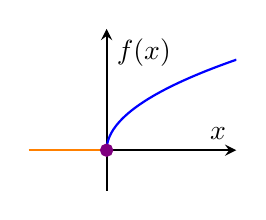
\begin{tikzpicture}
    \begin{axis}[
        width = 120,
        axis lines=middle,
        xlabel=$x$, ylabel=$f(x)$,
        samples=200,
        domain=-3:5,
        ymin=-1, ymax=3,
        xmin=-3, xmax=5,
        grid=both,
        thick, 
        xtick =\empty,
        ytick=\empty
    ]
    
    % Plot f(x) = 0 for x < 0
    \addplot[orange, thick, domain=-3:0] {0};
    
    % Plot f(x) = sqrt(x) for x >= 0
    \addplot[blue, thick, domain=0:5] {sqrt(x)};
    
    % Closed circle at (0,0) because both pieces agree
    \addplot[only marks, mark=*, mark size=2pt, violet] coordinates {(0,0)};
    
    \end{axis}
\end{tikzpicture}
